\begin{figure}[htbp]
	\centering
	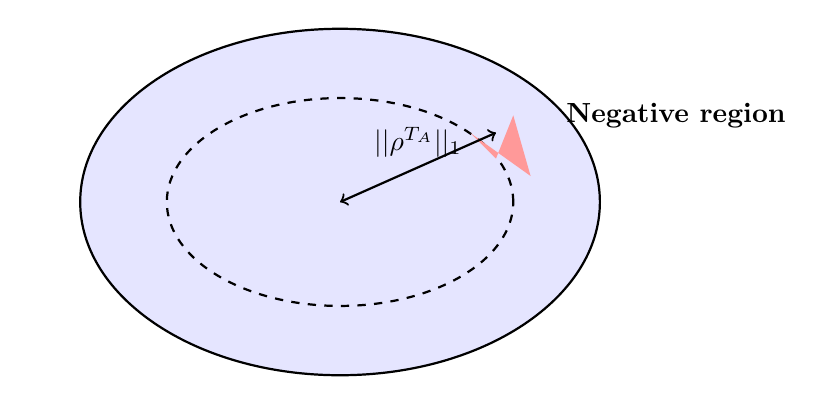
\begin{tikzpicture}[scale=1.1]
		\draw[thick, fill=blue!10] (0,0) ellipse (3cm and 2cm);

		\draw[thick, dashed] (0,0) ellipse (2cm and 1.2cm);

		\fill[red!40] (1.5,0.8) -- (2.2,0.3) -- (2.0,1.0) -- (1.8,0.5) -- cycle;

		\node at (-3.5,0) {
			% \begin{tabular}{p{3cm}}
			% 	\textbf{Partial transpose} \\
			% 	$\rho^{T_A}$
			% \end{tabular}
		};

		\node[right] at (2.5,1) {\textbf{Negative region}};

		\draw[<->, thick] (0,0) -- (1.8,0.8) node[midway, above] {$||\rho^{T_A}||_1$};

	\end{tikzpicture}
	\caption{Negativity visualization: the partial transpose $\rho^{T_A}$ of an entangled state has negative eigenvalues (shown in red). The negativity $N(\rho)$ measures the total "volume" of these negative regions, providing a quantifier of bipartite entanglement. Negativity $N(\rho) = \frac{||\rho^{T_A}||_1 - 1}{2}$: The "volume" of negative eigenvalues in the partial transpose indicates entanglement. For separable states, all eigenvalues are positive; for entangled states, negative eigenvalues appear.}
	\label{fig:negativity-visualization}
\end{figure}
